\chapter{Aplicações web com MEAN Stack}	 
\label{implementacao}

%\section{Aplicação Math Race  desenvolvido com outras tecnologias}

    O capítulo \ref{tecnologias} tinha como função apresentar cada elemento do MEAN Stack individualmente, neste capítulo vamos juntá-las para formar a pilha (Stack) e analisá-las em conjunto.
    
A figura \ref{fig:MEAN Stack visto como uma pilha} ilustra a pilha que é formada unindo as tecnologias já explicadas no capítulo anterior, no banco de dados coloca-se o MongoDB, no lado do servidor temos o Node.js e o Express e por último no lado do cliente o AngularJS, a seta de duplo sentindo representa que a passagem de dados acontece em ambos os sentidos. O principal motivo para estas tecnologias funcionarem bem em conjunto é que todas elas tem como base a linguagem Javascript, sendo que esta característica faz parte da proposta do MEAN que é o desenvolvimento de aplicações web escaláveis com a utilização de um Stack de ferramentas em Javascript.
    
\begin{figure}[htb]
\centering
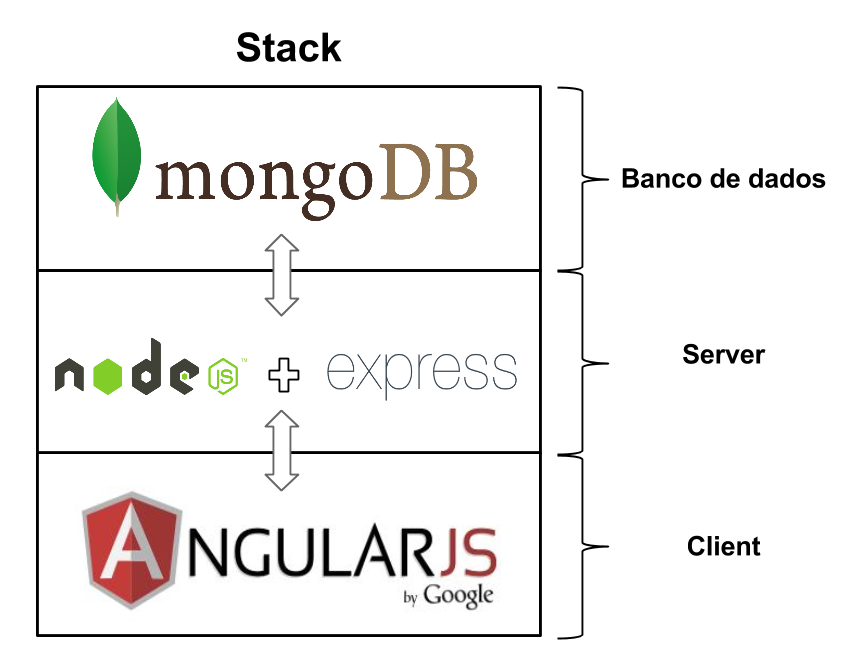
\includegraphics[scale=0.4]{images/mean_stack_diagram.png}
\caption{MEAN Stack visto como uma pilha}
\label{fig:MEAN Stack visto como uma pilha}
\end{figure}
    
\section{Comparativo em relação a arquitetura de aplicações LAMP}     
    Para cada componente da pilha existe uma quantidade razoável de tecnologias semelhantes, se utilizarmos  como exemplo a figura \ref{fig:Gráfico Comparando Frameworks Javascript} do capítulo \ref{tecnologias} da seção sobre AngularJS podemos observar uma grande quantidade de tecnologias concorrentes que existem, cada uma se destaca em alguma situação. Neste cenário se torna muito complicado concluir o que é melhor, ainda mais que o próprio MEAN pode variar, por exemplo para PEAN quando o MongoDB é substituído pelo PostgreSQL. 
    A comparação do MEAN será feita com o LAMP, pois este tem um destaque quando o assunto se trata de aplicações web. \cite{meanVSlamp}
   
   Assim como o MEAN, o LAMP é uma pilha de software livres como o foco no desenvolvimento web. A sigla LAMP é um acrônimo de Linux, Apache, MySQL e Pearl/PHP/Python.
   
   Uma característica que difere os dois stacks é que o LAMP, necessita do Linux, ou outro sistema operacional de qualquer forma ele fica preso a isso. Enquanto o MEAN pode ser executada em qualquer plataforma.
   
    O servidor do MEAN é o Node.js, enquanto ao do LAMP é Apache, o que destaca o Node.js neste caso é o fato de ser totalmente não bloqueante e ser orientado a eventos, como já citado na subseção 3.1.4, o que permite concorrência entre as requisições. Porém como o Node.js é recente não existe muitos plugins que auxiliam seu uso, o que não acontece com o Apache que já está há muito tempo  no mercado, sem dizer que em muitos casos ele é escolhido como servidor padrão de muitos desenvolvedores.
    
    O Banco de dados do MEAN é o MongoDB, que como já explicado anteriormente é um NoSQL, já o do LAMP é o MySQL que é um banco de dados SQL. A comparação entre esses bancos de dados deve-se considerar a situação, por exemplo uma consulta com intuito de retornar um valor no MongoDB é mais rápida do que no MySQL, pois o MongDB não possui schemas de tabelas mas sim um arquivo json. Em contra partida a atualização dos dados do banco pode ser muito lento para o MongoDB, isso considerando que temos muitos dados armazenados no banco.
    
    Por ultimo temos front-end no MEAN que é o AngularJS e o back-end no LAMP, que fica por conta de uma dessas tres liguagens de programaçao: Pearl,PHP ou Python. 
    No MEAN, express serve como a camada de controle, empacotando os dados e enviando para AngularJS que utiliza a informação para realizar alguma ação e renderizar a página. A principal vantagem de se utilizar o AngularJS é que ele é totalmente clientside, como já explicado no capitulo anterior.
    Todas as caracteristicas citadas nesta secção podem ser observada de forma mais direta na tabela da \ref{fig:tabela mean vs lamp}.
    
    O fato de todas as tecnologias do MEAN serem em javascripts garantem que o desenvolvedor precise saber apenas uma linguagem de programação, porém isso também tem seu lado negativo que é o engessamento do projeto só em Javascript, ou seja seu projeto fica dependente apenas do que o Javascript consegue fazer.
    
    \begin{figure}[htb]
    \centering
    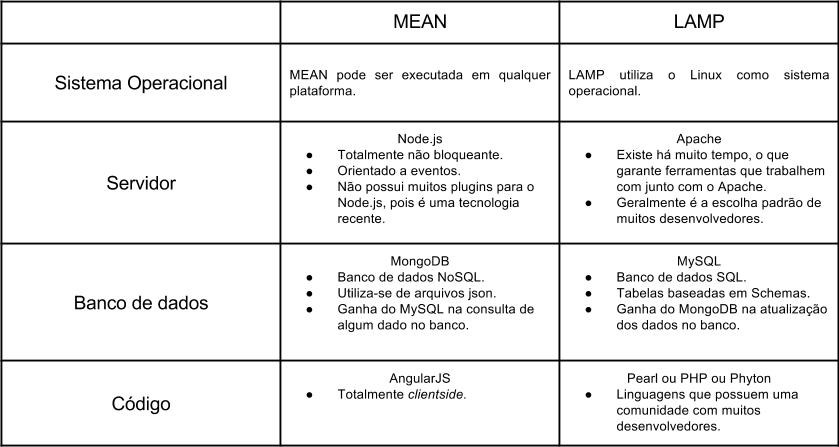
\includegraphics[scale=0.5]{images/mean_vs_lamp.png}
    \caption{Tabela de comparação entre MEAN vs LAMP}
    \label{fig:tabela mean vs lamp}
    \end{figure}
   
\section{Aplicação \textit{Math Race} com MEAN Stack}

Neste capítulo será apresentada uma aplicação desenvolvida com o MEAN Stack. A seção \ref{subsec: Proposta de desenvolvimento} descreve a proposta de desenvolvimento da aplicação. A seção \ref{subsec: Utilização e funcionamento da aplicação} mostra como é a utilização e o funcionamento da aplicação. A seção \ref{subsec: Desenvolvimento da aplicação} aborda como foi desenvolvida a aplicação. A seção \ref{subsec: Testes de desempenho} contém os testes de desempenho realizados.

\subsection{Proposta da aplicação}
\label{subsec: Proposta de desenvolvimento}
 Uma aplicação simples foi desenvolvida com o intuito de demonstrar diversos aspectos do MEAN Stack, como o desempenho e como funcionamento da integração das ferramentas que compõem o MEAN Stack. A aplicação foi baseada na implententação do Math Race desenvolvida por Iván Loire\cite{MathRace}, que possui apenas o Node.js e o Socket.io como ferramentas em comum.

\subsection{Utilização e funcionamento da aplicação}
\label{subsec: Utilização e funcionamento da aplicação}
 A aplicação é um jogo cujo objetivo é realizar uma competição em tempo real para ver qual jogador acertar mais operações de matemáticas aleatórias de adição e subtração em determinado tempo.

Na figura \ref{fig:Imagem da interface da aplicação} é mostrada a interface da aplicação, que contém a operação aleatória e o campo para entrada de dados, além do marcador de tempo, o campo de pontuação (\textit{score}) e o Hall da fama (\textit{Hall of fame}).

    \begin{figure}[htb]
    \centering
    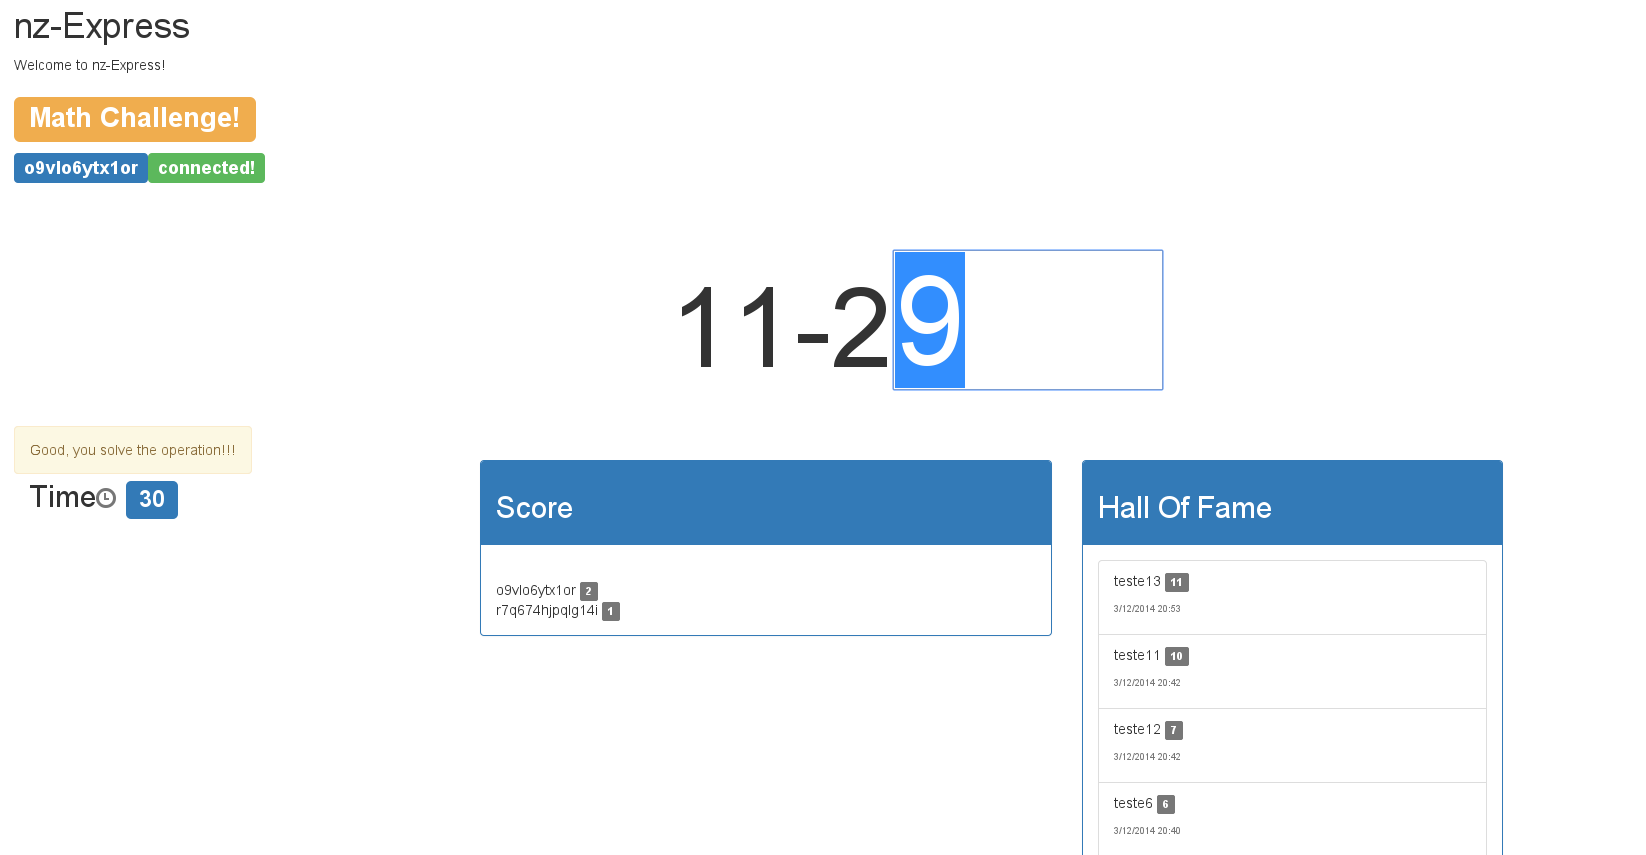
\includegraphics[scale=0.3]{images/index_mean_math_race.png}
    \caption{Imagem da interface da aplicação}
    \label{fig:Imagem da interface da aplicação}
    \end{figure}
    
Todos os jogadores possuem o mesmo tempo para responder a mesma operação matemática, o diferencial está em que a operação muda para todos os jogadores após a resposta correta da operação anterior ter sido preenchida por qualquer jogador.

O jogo funciona através de rodadas, e para cada rodada o usuário tem um tempo limite pré-determinado para acertar o resultado da conta, e a cada resultado correto o valor da pontuação do usuário, que começa em zero, é incrementado com mais um ponto. Ao final de uma rodada os usuários que efetuaram alguma pontuação são adicionados no ``Hall da fama'', que é ordenado pelos dez usuários com mais pontos obtidos em uma única rodada, e as pontuações dos usuários são zeradas para que uma nova rodada se inicie. 

% diagramas explicando o funcionamento da app 

\subsection{Desenvolvimento da aplicação}
\label{subsec: Desenvolvimento da aplicação}

\begin{description}
\item[Estrutura de arquivos] \hfill \\
No início do desenvolvimento da aplicação verificamos as possibilidades em relação a estrutura  organização de arquivos que seria utilizada, pois não exite uma abordagem padrão em relação a este assunto.

Nas pesquisas iniciais as primeiras possibilidades que apareceram foram através do MEAN.js e o MEAN.io que são geradores automáticos de estruturas de arquivos para o MEAN Stack. Apesar de fornecerem uma estrutura pronta, ao lidar com geradores é necessário que se programe de uma maneira pré-determinada de acordo com o gerador escolhido, o que torna a aplicação um pouco mais complexa de ser apresentada e detalhada, e foge do escopo desta monografia.

A opção escolhida para a criação da estrutura de diretórios foi através de um submódulo do Express chamado express-generator. A figura \ref{fig: estrutura criada pelo express-generator} \cite{ExpressGen} mostra como as pastas e os arquivos são organizados neste gerador, ao total temos 7 pastas e 9 arquivos. 

    \begin{figure}[htb]
    \centering
    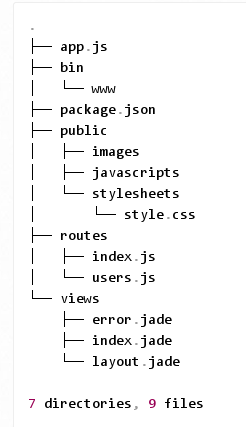
\includegraphics[scale=0.7]{images/estrutura_exp_gen.png}
    \caption{Estrutura criada pelo express-generator}
    \label{fig: estrutura criada pelo express-generator}
    \end{figure}

A pasta \textit{public} contém todos os arquivos de imagem, Javascript e CSS que serão enviados para o cliente, como por exemplo os arquivos javascript do Angular.js e o arquivo CSS chamado style.css.

Na pasta \textit{views} são definidas as páginas da aplicação, contendo a página do layout, do index, e uma página de erros, quando o usuário acessa a aplicação primeiramente é carregada a página de layout, que então carrega a página index, e caso algum erro ocorra ao invés da página de layout é carregado a página de erro.

Para as rotas, que definem como serão tratadas as requisições que podem ser realizadas pela aplicação, o express-generator cria uma pasta chamada \textit{routes}, que ao receber requisições pode desde renderizar as páginas solicitadas, até encaminhar as requisições para outras rotas afim de por exemplo realizar uma consulta em um banco de dados.

A parte do servidor que o Node.js é responsável fica no arquivo www da pasta \textit{bin}, e no arquivo app.js na raiz da aplicação.  

Além da estrutura criada pelo express-generator foram criadas mais duas pastas, que são a \textit{models} e a \textit{lib}. Na \textit{models} ficam os arquivos responsáveis pela conexão e pelos acessos ao MongoDB. A \textit{lib} contém as principais funções da aplicação responsáveis pelo funcionamento do jogo Math Race, e da comunicação Cliente/Servidor que é através do Socket.io.

\item[Integração das ferramentas do MEAN Stack] \hfill \\
Quando o usuário acessa a aplicação ocorrem uma série de mensagens, entre o lado do cliente e do servidor, afim de informar o servidor que há um novo usuário conectado e fazer com que o cliente obtenha os dados da partida. 

A figura \ref{fig: Diagrama de sequência do acesso da aplicação} demonstra a sequência de mensagens que ocorrem quando qualquer usuário acessa a aplicação (mensagem 1). 

No lado do servidor, o Node.js envia os arquivos da pasta \textit{public} e o \textit{index} da aplicação (mensagem 2). No lado do cliente, o Angular.js envia uma solicitação de conexão através da função \textit{connect} do Socket.io (mensagem 3), e o Node.js responde com uma mensagem avisando que o usuário está conectado (mensagem 4), ao receber esta mensagem o Angular.js envia outra mensagem chamada "\textit{join}" (mensagem 5), e o Node.js envia os dados referente a operação, a pontuação e o hall da fama (mensagem 6, 7 e 8). Por último o Angular.js faz um requisição ao MongoDB para obter o hall da fama atualizado (mensagem 9). 

    \begin{figure}[htb]
    \centering
    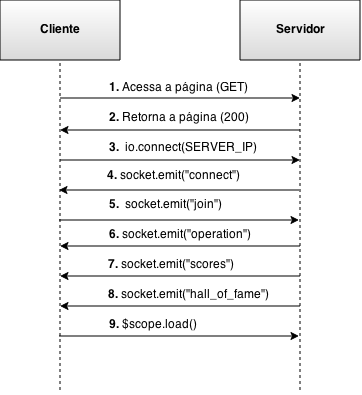
\includegraphics[scale=0.7]{images/diagrama_de_seq_acesso.png}
    \caption{Diagrama de sequência do acesso da aplicação}
    \label{fig: Diagrama de sequência do acesso da aplicação}
    \end{figure}
% codigo do join

A cada final de rodada o Node.js envia uma nova operação, e o Angular.js envia uma mensagem ao Node.js solicitando o Hall da fama atualizado, esta mensagem é enviado através de um módulo do Angular.js chamado ng-resource, e através deste módulo é possível interagir com o Node.js utilizando o RESTFul\footnote{ ``RESTful é um serviço web que utiliza o paradima de arquitetura do REST, ou seja, é o termo normalmente usado para se referir a implementação de Web Services que utilizam tal arquitetura.''\cite{RESTWiki}}. 

Caso o usuário tenha efetuado alguma pontuação na rodada, o Angular.js envia uma mensagem ao  Node.js contendo um objeto JSON com o nome e a pontuação efetuada. O Node.js então faz a inserção no MongoDB se for um novo usuário, ou atualiza a pontuação, se o nome do usuário já estiver cadastrado no MongoDB, e a pontuação for maior do que a que estava armazenada.

% diagrama demonstrando a aplicação em execução
\end{description}

% \begin{lstlisting}
% 	$scope.sendResult = function(item) {
% 		if (item.value) {
% 		    ...
% 			socket.emit('send-server-result', item);
% 		};
% 	}
% \end{lstlisting}

\subsection{Testes de desempenho}
\label{subsec: Testes de desempenho}
Nesta subseção o objetivo é demonstrar o comportamento da aplicação através de um conjunto de testes de envio de requisições e consultas ao banco de dados. 

Os testes foram realizados aumentando gradativamente a quantidade de requisições, afim de verificar a latência de resposta do servidor. A cada requisição é realizada uma consulta no banco de dados para obtenção da lista dos dez primeiros usuários e suas pontuações no hall da fama.

Na figura \ref{fig: Lista de objetos retornada pelo MongoDB} podemos observar parte da lista de objetos retornado pela consulta ao banco de dados realizadas no teste.

    \begin{figure}[htb]
    \centering
    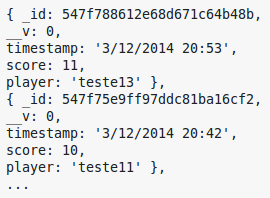
\includegraphics[scale=0.7]{images/objs_hof_bd.png}
    \caption{Lista de objetos retornada pelo MongoDB}
    \label{fig: Lista de objetos retornada pelo MongoDB}
    \end{figure}
% \begin{lstlisting}
%   { _id: 547f788612e68d671c64b48b,
%   __v: 0,
%   timestamp: '3/12/2014 20:53',
%   score: 11,
%   player: 'teste13' },
%   { _id: 547f75e9ff97ddc81ba16cf2,
%   __v: 0,
%   timestamp: '3/12/2014 20:42',
%   score: 10,
%   player: 'teste11' },
%   ...
%  \caption{Código}
% \end{lstlisting}

%figura do JSON retornado pelo MongoDB

A máquina utilizada nos testes tem como configurações um Core i7 de 3.6GHZ, e 8GB de memória RAM, utilizando o Fedora 20 de 64 \textit{bits} como sistema operacional.

\begin{table}[ht]
\centering
\begin{tabular}{|c|c|c|c|}
\hline
\# requisições concorrentes & \# requisições & tempo(seg) & req/seg      \\ \hline
\rowcolor[HTML]{EFEFEF} 
\cellcolor[HTML]{EFEFEF} & 1000 & 0,69 & 1458 req/s \\ \cline{2-4}
\rowcolor[HTML]{EFEFEF} 
\cellcolor[HTML]{EFEFEF} & 2000 & 1,357 & 1472 req/s \\ \cline{2-4}
\rowcolor[HTML]{EFEFEF} 
\cellcolor[HTML]{EFEFEF} & 5000           & 3,437      & 1454 req/s \\ \cline{2-4} 
\rowcolor[HTML]{EFEFEF} 
\cellcolor[HTML]{EFEFEF} & 10000          & 7,690      & 1414 req/s \\ \cline{2-4} 
\rowcolor[HTML]{EFEFEF} 
\cellcolor[HTML]{EFEFEF} & 30000          & 20,928     & 1433 req/s \\ \cline{2-4} 
\rowcolor[HTML]{EFEFEF} 
\cellcolor[HTML]{EFEFEF} & 50000          & 34,986     & 1429 req/s \\ \cline{2-4} 
\rowcolor[HTML]{EFEFEF} 
\cellcolor[HTML]{EFEFEF} & 70000          & 47,102     & 1486 req/s \\ \cline{2-4} 
\rowcolor[HTML]{EFEFEF}
\multirow{-8}{*}{\cellcolor[HTML]{EFEFEF}100} & 100000 & 67,967     & 1471 req/s \\ \hline
    & 1000           & 3,250      & 330 req/s  \\ \cline{2-4} 
    & 2000           & 1,385      & 1443 req/s \\ \cline{2-4} 
    & 5000           & 3,691      & 1354 req/s \\ \cline{2-4} 
    & 10000          & 7,503      & 1332 req/s \\ \cline{2-4} 
    & 30000          & 21,963     & 1365 req/s \\ \cline{2-4} 
    & 50000          & 37,327     & 1339 req/s \\ \cline{2-4} 
    & 70000          & 52,157     & 1342 req/s \\ \cline{2-4} 
\multirow{-8}{*}{1000}   & 100000         & 74,914     & 1334 req/s \\ \hline    
\end{tabular}
\caption{Carga na quantidade requisições}
\end{table}

    \begin{figure}[htb]
    \centering
    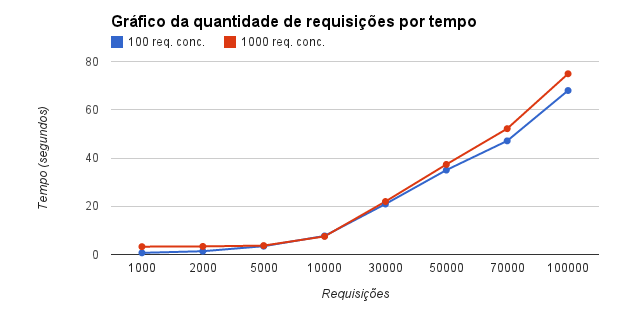
\includegraphics[scale=0.7]{images/reqxtempo.png}
    \caption{Gráfico de requisições por tempo}
    \label{fig: Gráfico de requisições por tempo}
    \end{figure}

\begin{table}[ht]
\centering
\begin{tabular}{|c|c|c|c|}
\hline
\# requisições & \# requisições concorrentes & tempo(seg) & req/seg \\ 
\hline
\rowcolor[HTML]{EFEFEF} 
\cellcolor[HTML]{EFEFEF}    & 100      & 0,664      & 1504  \\ \cline{2-4} 
\rowcolor[HTML]{EFEFEF} 
\cellcolor[HTML]{EFEFEF}    & 500      & 1,550      & 947   \\ \cline{2-4} 
\rowcolor[HTML]{EFEFEF} 
\multirow{-3}{*}{\cellcolor[HTML]{EFEFEF}1000}  & 1000     & 3,400      & 328   \\ \hline
        & 100      & 3,321      & 1505  \\ \cline{2-4} 
        & 500      & 3,479      & 1436  \\ \cline{2-4} 
\multirow{-3}{*}{5000}      & 1000     & 3,514      & 1422  \\ \hline
\rowcolor[HTML]{EFEFEF} 
\cellcolor[HTML]{EFEFEF}    & 100      & 6,760      & 1479  \\ \cline{2-4} 
\rowcolor[HTML]{EFEFEF}
\cellcolor[HTML]{EFEFEF}    & 500      & 7,200      & 1428  \\ \cline{2-4} 
\rowcolor[HTML]{EFEFEF} 
\multirow{-3}{*}{\cellcolor[HTML]{EFEFEF}10000} & 1000 & 7,201 & 1388  \\ \hline
        & 100      & 10,581     & 1417  \\ \cline{2-4} 
        & 500      & 11,170     & 1361  \\ \cline{2-4} 
\multirow{-3}{*}{15000}     & 1000     & 11,560     & 1356  \\ \hline
\rowcolor[HTML]{EFEFEF} 
\cellcolor[HTML]{EFEFEF}    & 100      & 16,863     & 1482  \\ \cline{2-4} 
\rowcolor[HTML]{EFEFEF}
\cellcolor[HTML]{EFEFEF}    & 500      & 17,849     & 1400  \\ \cline{2-4} 
\rowcolor[HTML]{EFEFEF}
\multirow{-3}{*}{\cellcolor[HTML]{EFEFEF}25000} & 1000 & 18,535 & 1348  \\ \hline
        & 100      & 20,371     & 1472  \\ \cline{2-4} 
        & 500      & 21,662     & 1384  \\ \cline{2-4} 
\multirow{-3}{*}{30000}     & 1000     & 22,405     & 1338  \\ \hline
\end{tabular}
\caption{Carga na quantidade requisições concorrentes}
\end{table}

    \begin{figure}[htb]
    \centering
    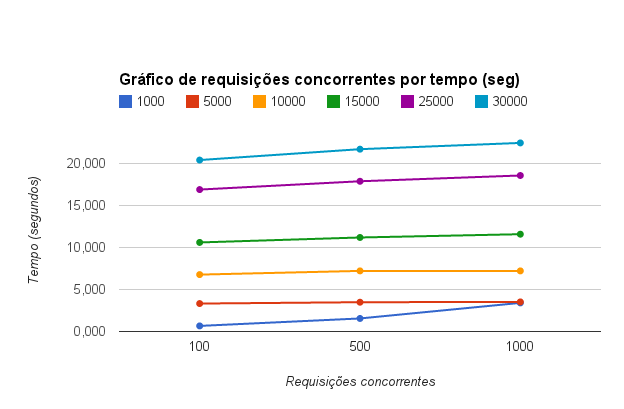
\includegraphics[scale=0.7]{images/req_conc_tempo.png}
    \caption{Gráfico de requisições concorrentes tempo}
    \label{fig: Gráfico de requisições concorrentes por tempo}
    \end{figure}
% a tabela/grafico XXX mostra os testes de carga de requisições

%de maneira pura, ou seja, sem que haja alteração para obtenção de resultados  



% PROPOSTA DE DESENVOLVIMENTO

% DIAGRAMA DE CASOS DE USO
%  Especificações dos cs

% DESENVOLVIMENTO DA APLICAÇÃO

% UTILIZAÇÃO DA APLICAÇÃO

%  TESTES DE DESEMPENHO
%   weigthttp
%   objetivo do teste, como foram realizados, hardware utilizado
%      analise dos resultados obtidos

%   figura

% analise dos teste

